\section{Números Reales}
%%%%%%%%%%%%%%%%%%%%%
\subsection{Conjuntos numéricos}
{Números naturales}
	\begin{align*}
		\N = \set{0,1,2,3,...}
	\end{align*}

%%%%%%%
{Números enteros}
	\begin{align*}
		\Z = \set{0,\pm1, \pm 2,...}
	\end{align*}

%%%%%%%
{Números racionales}
	\begin{align*}
		\Q = \sett{\dfrac{p}{q}}{p,q\in Z, q\neq 0}\Big/\sim
	\end{align*}

%%%%%%%
{Equivalencia de fracciones}
	\begin{align*}
		\dfrac{a}{b}\sim \dfrac{c}{d} \iff ad-bc=0 
	\end{align*}

%%%%%%%
{Números irracionales}
	Existen números en la recta numérica que no se pueden representar como fracciones.
	
	Por ejemplo $\sqrt{2}, e, \pi...$.

%%%%%%%
{}
\begin{figure}
 \centering
 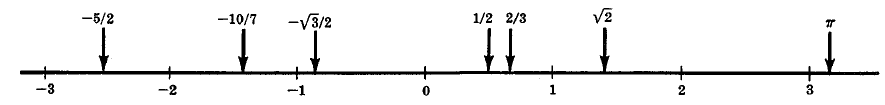
\includegraphics[width=.8\textwidth]{./calculo/fig-01-01--recta_numerica.png}
 % fig-01-01--recta numérica.png: 885x105 px, 120dpi, 18.73x2.22 cm, bb=0 0 531 63
 \label{fig:schaum 01 01}
\end{figure}


%%%%%%%
{Números reales}
	La unión de número racionales e irracionales se le conoce como \emph{números reales} $\R$.

%%%%%%%
\subsection{Orden}

	Los números reales se clasifican en
	\begin{itemize}
		\item Positivos $\set{x\in \R| x>0}$ 
		\item Cero $\set{0\in \R}$ 
		\item Negativos $\set{x\in \R | x<0}$
	\end{itemize}

%%%%%%%

 Diremos que $b\in \R$ es mayor que $a\in\R$ si $b-a>0$. 
  
 
 En ese caso escribimos $b>a$.

%%%%%%%
{}
	Diremos que $a\in \R$ es menor que  $b\in\R$ si $a-b<0$.
	
	En ese caso escribimos $a<b$.

%%%%%%%
{}
	\begin{proposicion}
		\begin{align*}
		b>a \iff a<b	
		\end{align*}
	\end{proposicion}

%%%%%%%
{Desigualdades}
	\begin{proposicion}
		Sean $a,b\in\R$. Entonces se cumple una y solo una de las siguientes condiciones:
		\begin{itemize}
			\item $a>b$
			\item $a=b$
			\item $a<b$
		\end{itemize}
	\end{proposicion}

%%%%%%%
\subsection{Reglas de álgebra}
%\subsection{Axiomas}

	Para cualesquiera $a,b,c\in\R$, se tienen las siguientes propiedades:

%%%%%%%
{}
	\begin{axioma}[Conmutatividad de la suma]
		\label{axiom--1}
		\begin{align*}
		a+b=b+a
		\end{align*}
	\end{axioma}

%%%%%%%
{}
	\begin{axioma}[Asociatividad de la suma]
		\label{axiom--2}
		\begin{align*}
	(a+b)+c = a+(b+c)
		\end{align*}
	\end{axioma}

%%%%%%%
{}
	\begin{axioma}[Conmutatividad del producto]
		\label{axiom--3}
		\begin{align*}
		ab=ba
		\end{align*}
	\end{axioma}

%%%%%%%

{}
	\begin{axioma}[Asociatividad del producto]
		\label{axiom--4}
		\begin{align*}
		(ab)c = a(bc)
		\end{align*}
	\end{axioma}

%%%%%%%
{}
	\begin{axioma}[Ley de la distribución]
		\label{axiom--5}
		\begin{align*}
		a(b+c)=ab+ac
		\end{align*}
	\end{axioma}

%%%%%%%
{Leyes de los exponentes}
	\begin{itemize}
		\item $a^{m}\cdot a^{n} = a^{m+n}$ 
		\item $\dfrac{a^{m}}{a^{n}} = a^{m-m}, a\neq 0$ 
		\item $\left(a^{m}\right)^{n} = a^{mn}$
	\end{itemize}


	\begin{itemize}
		\item $ a^{1}= a $ 
		\item $ a^{0}= 1 $ 
		\item $ a^{-1}= \dfrac{1}{a} $ 
		\item $ a^{n}= \dfrac{1}{a^{n}}  $
		\item $ a^{p/q}= \sqrt[q]{a^{p}} $
	\end{itemize}

\subsection{Ejemplos}

{}
 \begin{problema}
 	Demuestra que $\sqrt{2}$ es un número irracional.
 \end{problema}

%%%%%%%
{Solución}
	Procedamos por contradicción: 
	\begin{enumerate}
		\item Supongamos que $\sqrt{2}=\dfrac{p}{q}$ con $ p,q \in \Z$ positivos y primos relativos.  
		\item Entonces $ 2= \dfrac{p^{2}}{q^{2}}$, de manera que $p^{2}=2q^{2}$.
		\item De manera que $p$ es par, es decir, existe un entero $m$ tal que $p=2m$. 
		\item Sustituyendo obtenemos que $q^{2}=2m^{2},$ de manera que $q$ también es par. 
		\item Pero por hipótesis, $p$ y $q$ son primos relativos, de manera que no pueden ser ambos pares. $\qed$
	\end{enumerate}


%%%%%%%
{}
	\begin{problema}
		¿Qué número es más grande: $\sqrt{2}$ o $ \sqrt[3]{3} $?
	\end{problema}

%%%%%%%
{Solución}
	Procedamos por contradicción:
	\begin{enumerate}
		\item 
		Supongamos que $ \sqrt{2} \geq \sqrt[3]{3}$. 
		\item Elevamos ambos lados a la sexta potencia. 
		\item De donde obtenemos que 
		\begin{align*}
			2^{3} \geq 3^{2} \qed
		\end{align*} 
	\end{enumerate}

%%%%%%%
{}
	\begin{problema}
		Con base en los axiomas \eqref{axiom--1}-\eqref{axiom--5}, demostrar que
		\begin{align*}
			(b+c)a=ba+ca
		\end{align*}
	\end{problema}

%%%%%%%
{Solución}
		\begin{align*}
		(b+c)a &= a(b+c)\\ 
		&=ab+ac \\ 
		&=ba+ca
		\end{align*}

